% # Introduction

%---

% \subsection{Old Intro}

% Robot learning of manipulation policies in the open world -- in situations, and to objects, the robot has not previously encountered -- is a grand challenge in robotics. An important aspect of this problem is our representation of the 3D world. Our paper focuses on a factored representation of the world, where we first find all objects of interest and then represent the 3D shape of each object independently. Our representation should generalize to unfamiliar objects in unfamiliar environments. For example, a robot should be able to enter a new kitchen and place a mug of a new shape on a hook (Figure \ref{fig:intro}). Additionally, we wish the robot to generalize to objects placed in novel positions and orientations. E.g. the robot should be able to pick a mug laying sideways on a floor even if it has previously only seen mugs standing on a countertop. We call this property $\mathrm{SE}(3)$-equivariance.

% Classical robotics approaches represent objects using explicit 3D geometries. \citet{miller03automatic,tenorth13decomposing} decompose complex objects into primitive shapes to plan for grasps and \citet{klank09realtime,beetz11robotic} rely on having CAD models of all objects in the world. The generalization ability of these approaches is limited, as these hand-crafted 3D representations cannot be accurately fit to any new object the robot encounters. To address this limitation, recent approaches use implicitly learned 3D descriptors. \citet{mescheder19occupancy,park19deepsdf} represent the 3D surface of an object as a decision boundary of a binary classifier neural network. Each 3D point nearby the surface of the object can then be described using the activations of the neural network \cite{simeonov22neural}. \citet{pan22taxpose} use neural point cloud embeddings \cite{qi17pointneta} and cross-attention \cite{vaswani17attention} to learn point cloud representations that are comparable between object instances.

% Implicit 3D descriptors have led to impressive results in few-shot 3D manipulation. Neural Descriptor Fields (NDFs) \cite{simeonov22neural,simeonov22se} and TAX-Pose \cite{pan22taxpose} learn object re-arrangement policies, e.g. hanging a mug on a hook, from 5 - 10 demonstrations. NDFs use 3D descriptors to match task-relevant object parts between different instances of objects. For example, they align the handles of differently shaped mugs in order to successfully hang them. Alternatively, Tax-Pose computes the cross-attention between the child (mug) and the parent (hook) objects in order to find which parts of the two objects should be nearby each other in the target configuration (mug on tree). The direct comparison between the child and the parent objects can lead to higher accuracy than in NDFs. But, both NDFs and Tax-Pose have two important limitations: (1) a large collection of 3D meshes is required for pre-training (200 objects per category from ShapeNet \cite{chang15shapenet}) and (2) without explicit 3D geometries, it is difficult to perform collision checking and motion planning on a physical robot.

% Our paper focuses on an alternative and highly sample-efficient explicit 3D geometry representation method based on \textit{shape warping} \citep{jakel12learning,brandi14generalizing,lee15learning,schulman16learning,rodriguez18transferring,rodriguez18transferringa,thompson21shapebased}. The core idea is to pick a canonical example of an object class, and warp its point cloud (or mesh) to conform to the observations of novel object instances \cite{myronenko10pointset,hillenbrand12transferring,benamor12generalization}. The immediate benefit is that we do not have to represent the shape of an object, but only the \textit{displacement} of points as they are warped between different object instances (belonging to the same object class). We base our method on prior work by \citet{rodriguez18transferring,thompson21shapebased}, who propose to use gradient-descent-based inference to enable shape warping to partial point clouds.
% % \tk{We base our method on ... [or mention this connection later in the method section, might not be needed here]} 

% We propose \textbf{Shape and Action Warping (SA-Warp)}, a general method for one-shot learning of robotic manipulation policies. First, we propose a new algorithm for the joint inference of object shape, scale, translation and orientation based on its partial point cloud. The algorithm is based on canonical object warping with a low-dimensional latent space of shapes \cite{rodriguez18transferring,thompson21shapebased} and returns a warped 3D mesh. Second, we propose a method for the warping of robot actions. We focus on actions where two objects come into contact: e.g., grasping, relative object placement (e.g. mug on tree) and trajectory cloning with contacts (e.g. painting with a brush on a canvas). Our method finds the \textit{interaction points} between pairs of objects, anchors them to their canonical counterparts, and warps them to conform to objects of novel shapes. We developed SA-Warp specifically for on-robot behavior cloning, and we extensively test it in real-world robot experiments.

%---

% Our first contribution is an algorithm for the joint inference of the shape and pose of an object from its partial point cloud. We jointly optimize the shape, scale, position and orientation of a canonical object to match the observed point cloud. We show our method is $\mathrm{SE}(3)$-invariant in the limit of random restarts. We also propose a simple method for turning the inferred point cloud into meshes. Our second, and more important, contribution is the warping of robot actions. We focus on actions where two objects come into contact: e.g., grasping, relative object placement (e.g. mug on tree) and trajectory cloning with contacts (e.g. painting with a brush on a canvas). We identify the \textit{interaction points} between a pair of objects. For grasps, those are the pairs of contact points between the gripper and the target object. 

%For robotic grasping, we identify the \textit{contact points} between the gripper and the target object. We register the contacts points on the canonical mesh of our target object class, and warp them to conform to novel object instances. For example, our algorithm alters the pose of the gripper in order to grasp the rim of a mug based on how tall the mug is and what its orientation is. For object placement and trajectory cloning, we identify pairs \textit{nearby points} between the pair of objects (e.g. a mug and a tree). We anchor the points on the canonical counterparts of the pair of objects, and solve for the relative pose of a new pair of objects using a pairwise best fit algorithm.

%We broaden the shape warping paradigm to include the \textit{warping of actions}. Instead of matching descriptors attached to 3D points (NDFs), or computing cross-attention between point clouds (TAX-Pose), we warp the pick and place poses, shown in a single demonstration of a task, to conform to novel object shapes. Specifically, for pick actions, we select a point on the canonical object closest to the contact between the gripper and the object. The position of the gripper translates as the canonical object grows and shrinks during warping, and the pose of the gripper rotates with the object. For place action cloning \evdp{action place cloning has not been introduced yet}, we identify pairs of \textit{contact points} between the pair of objects involved in the action, e.g. a mug and a mug-tree, or a mug and the ground. The contact points transform as their parent object is warped, and a new target pose is computed to connect the pairs of warped contact points as closely as possible. Our method is $\mathrm{SE}(3)$ equivariant, as the demonstrated pick and place actions are registered on the canonical object instance in a canonical reference frame. When we warp pick actions and place contact points to novel object instances, we again do so irrespective of to the pose of the objects. Object pose only affects our ability to perceive them \evdp{what does `them' refer to?}, as we work with partial point clouds.
%\lsw{Readers unlikely familiar with equivariance, go gentle. There are some important points here that are worth more sentences. (Also why is this paragraph repeated?)}

%We contribute a new inference method for SST-W \cite{thompson21shapebased} \evdp{add short description of new inference method} and a novel pick-and-place warping method that leverages canonicalization.
%\lsw{With all due credit and respect to Rory, this might be underselling because it sounds like you created a small extension specific to a niche method. A bolder move is to just claim a new method, and then later qualify (as you have in Section IV-B) that you build on SST-W.}
%Unlike prior work, we require only five to ten examples of an object class to learn our object representation. We perform real-world experiments on X $\mathrm{SE}(3)$ pick-and-place tasks using a full perception and motion planning pipeline described in section Y. We find Z. We also isolate the problem of relative pose prediction (as done in prior work \cite{pan22taxpose,simeonov22neural}), and run a comparison in simulation.

% Any robot deployed in the world can expect to encounter things it has not seen before, and an effective robot should be able to manipulate them. For instance, in an unfamiliar home, a robot should be able to hang an unfamiliar mug on an unfamiliar hook. \tk{Maybe say something about how representing the 3D world really matters for robotics, i.e. a bit more of a general statement before you go into the specific example of object shape generalization} To do so, a robot has to generalize over object shapes and manipulate objects in any 3D position and orientation. It should also generalize to a re-arrangement of objects in a scene, a property we call $\mathrm{SE}(3)$-equivariance. \evdp{re-arrangement of objects in a scene seems more related to decomposition/permutation/factorization generalization, not SE3 equivariance}\tk{+1, I think a better example could be that it should e.g. be able to generalize to a mug placed sideways on the floor, even though it only ever saw demonstrations for mugs placed upright on a table or counter}

%Classical robotics approaches use primitive shapes \citep{miller03automatic,tenorth13decomposing} or fully-specified CAD models \citep{klank09realtime,beetz11robotic} to model objects, and describe the world and tasks using symbolic models with limited scope \citep{kaelbling11hierarchical,bartels13constraintbased} \evdp{vague, how and why is the scope limited?}. Hence, their generality is limited. Recently, deep learning methods have begun to make inroads in this problem by employing large generalizable networks trained on similarly large datasets []. While deep learning systems learn impressive policies, they are often limited to top-down manipulation \citep{levine18learning,zhu22sample} \tk{Maybe have a short sentence explaining what top-down manipulation means?} and can require thousands of interactions with specific object instances \citep{yu19metaworld,wang22mathrmso}.%, and sometimes involve learning with only low-level percepts, such as object positions and velocities, unable to generalize to novel objects \citep{haarnoja18Soft,li20Practical}.

%More recently, Neural Descriptor Fields (NDFs) \cite{simeonov22neural,simeonov22se} and TAX-Pose \cite{pan22taxpose} achieved sample-efficient learning of $\mathrm{SE}(3)$-equivariant object re-arrangement policies. These methods assume the ability to segment objects in a scene, allowing them to focus on representing the shapes of individual objects. Shape representations are learned with deep point cloud \cite{qi17pointnet,qi17pointneta} or mesh \cite{mescheder19occupancy,park19deepsdf} encoders using on the order of hundreds of example object meshes per object class \cite{chang15shapenet}. The key to sample-efficiency of NDFs and TAX-Pose is the ability to assign a descriptive feature vector to 3D points around the objects of interest. NDFs directly match target poses of objects across different instances using gradient descent, where TAX-Pose computes cross-attention between encodings of individual points in a point cloud. The matching of 3D features is learned from about 10 demonstrations of a particular task.

%These are used to either directly match target poses of objects across different instances \cite{simeonov22Neural,simeonov22Neurala}, or are further processed by cross-attention layers \cite{vaswani17Attention}. 

% 1. Importance of open-world pick-and-place; SE(3); deep learning might make it possible, but i t's limited to closed domains,
% many demonstrations, lack of generalization.
% E.g. the original GNN factored block stacking paper doesn't even see the objects it manipulates.

% Among many desired capabilities, a robot should be able to generalize to novel instances of objects \evdp{can we add a concrete example?}, and should be able to synthesize pick-and-place actions in $\mathrm{SE}(3)$, enabling it to arrange objects in any position and orientation. Many past robotics works have tackled these challenges. 

%Yet, they were often limited to modeling objects using primitive shapes \citep{miller03Automatic,tenorth13Decomposing}, or fully-specified CAD models \citep{klank09Realtime,beetz11Robotic}, and describing the world and tasks using symbolic models with limited scope \citep{kaelbling11Hierarchical,bartels13Constraintbased}. % OB: Four of these papers are from the same German group, should diversify.

%% OB: Perhaps we don't need this paragraph.
%Recently, deep learning was posed to overcome these challenges with large generalizable neural networks trained on large datasets \citep{schmidhuber15Deep} \evdp{instead of a generic citation, you should add a bunch of citations of deep learning for robotics (/grasping)} \lsw{or a particularly recognizable survey paper}.
%While deep learning systems learn impressive policies,  they are often limited to top-down manipulation \citep{levine18Learning,zhu22Sample}, can require (at least) tens of thousands of interactions with specific object instances \citep{yu19MetaWorld,wang22MathrmSO}, and sometimes involve learning with only low-level percepts, such as object positions and velocities, unable to generalize to novel objects \citep{haarnoja18Soft,li20Practical}. % OB: SAC might not be the best citation here.

% 2. Object factorization and shape understanding can greatly improve sample efficiency.
% However, these approaches require large libraries of objects.
% Moreover, the way we extract feature vectors from all NN activations (do all models do this?) is tricky.

%\lsw{The following two paragraphs feel a bit like a related work section; on a related note, the intro is quite long.}
%Factoring scenes into individual object states \citep{janner19Reasoning,kipf20Contrastive} and representing the appearance of these objects using geometric deep learning methods \citep{mescheder19Occupancy,park19DeepSDF,mildenhall20NeRF,sajjadiObject} can greatly increase sample-efficiency and generality of robot learning systems. Recent works demonstrate class-level $\mathrm{SE}(3)$ manipulation learned from a handful of demonstrations \citep{simeonov22Neural,pan22TAXPose,simeonov22Neurala,wen22You}. The key to sample-efficiency of these methods is the ability to assign a descriptive feature vector to 3D points around the object of interest. These are used to either directly match target poses of objects across different instances \cite{simeonov22Neural,simeonov22Neurala}, or are further processed by cross-attention layers \cite{vaswani17Attention}. 

%\lsw{Write out the full name the first time you introduce something.}
%NDFs \citep{simeonov22Neural} assign a descriptor to an arbitrary point in 3D using a pre-trained Occupancy Network \cite{mescheder19Occupancy}, which contains information about the local geometry around the point. TAX-Pose \citep{pan22TAXPose} pre-train \ob{double-check} a point cloud encoder using contrastive learning \cite{oord19Representation}, so that the points corresponding to, for example, the handle of a mug have similar feature vectors across object instances. As a consequence, these methods require access to moderately large libraries of realistic CAD models \cite{chang15ShapeNet}.
%\lsw{Quantify what is ``moderately large''?}
%Further, spatial feature learning is still an open question; e.g., the concatenation of all intermediate neural activations of an Occupancy Network, as done in NDFs, is not a compact 3D point descriptor. Contrastive learning can be sensitive to the choice of negative samples \cite{biza21Impact}. % Could not resist the self cite :> 

% OB: How does "You Only Demonstrate Once" fit into this?

%Yet more recently, ... object-factorization [C-SWM, O2P2] ... object shape understanding [occupancy networks, deep sdfs, nerfs, osrts] ... highly sample-efficient SE(3) pick-and-place

% 3. In another line of work, shape warping has been used to clone grasps.
% These methods are limited to full point clouds and usually clone grasps only (not all I guess, there's the fabric manipulation paper).
% Recently, Skye proposed to learn a low-dimensional latent space that warps a canonical object, and fit it to new shapes using gradient descent.
% 4. We propose to use canonicalization for both shape warping and pick-and-place cloning. Given a single demonstration, we register the pick pose and the contact points between the held object and the target during placement. As the shape of the canonical object warps to conform to a new instance, the pick and place poses warp correspondingly.
% Additionally, we also warp the faces of the object, giving us a collision mesh for planning.
% Our method is $\mathrm{SE}(3)$ equivariant, as pick and place poses are predicted in a reference frame invariant to the current pose of the objects in the scene.

% We extend the shape warping paradigm to include the \textit{warping of actions}. Instead of matching descriptors attached to 3D points \citep{simeonov22Neural}, or computing cross-attention between point clouds \citep{pan22TAXPose}, we warp the pick and place poses, shown in a single demonstration of a task, to conform to novel object shapes. Specifically, for pick actions, we select a point on the canonical object closest to the contact between the gripper and the object. The position of the gripper translates as the canonical objects grows and shrinks during warping, and the pose of the gripper rotates with the object. For place action cloning, we identify pairs of \textit{contact points} between the pair of objects involved in the action, e.g. a mug and a mug-tree, or a mug and the ground. The contact points transform as their parent object is warped, and a new target pose is computed to connect the pairs of warped contact points as closely as possible. Our method is $\mathrm{SE}(3)$ equivariant, as the demonstrated pick and place actions are registered on the canonical object instance in a canonical reference frame. When we warp pick actions and place contact points to novel object instances, we again do so irresponsive \evdp{?} to the pose of the objects. Object pose only affects our ability to perceive them \evdp{what does `them' refer to?}, as we work with partial point clouds.

%we can both \textit{detect a class of object} and \textit{understand the intra-class shape variation} from few examples (around 10). 
% 1. Many prior SE(3) behavior cloning works do not use any pre-trained information about objects. Then, they need to see many demonstrations to understand both the task and the objects that are involved in it.
% 2. Prior object pre-training methods use large libraries of hand-crafted 3D meshes of objects. This approach would not work for specialized objects, e.g. in a manufacturing setting. \evdp{Why not? Could we craft 3D meshes of specialized objects?}
% 3. We propose a simple method based on warping pick locations and warping and matching contact points during object placement.
% \evdp{can you make a bullet list of contributions?}

% # Related work

% We build on a body of work in robotics that aims to learn generalizable manipulation policies from few demonstrations. A seminal idea in the literature is based on key-point representations of objects \evdp{cite the paper that introduced the idea}. \citet{manuelli19kpam} manually create a dataset of semantically meaningful key-points, such as the rim and the handle of a mug, and train a classifier to detect key-points on novel object instances. A task is defined as a time series of key-point positions. Then, a trajectory for a previously unseen object can be computed by matching the key-points on the novel object to the key-point positions seen in a demonstration. In comparison, our method does not require a manual labeling of key-points -- we use the inferred geometry of objects to automatically extract interaction points. \citet{gao21kpam,gao21kpamsc} further extend the key-point framework with feedback control and collision checking. Later works addressed key-point learning \cite{qin20keto,vecerik20s3k,manuelli20keypoints,turpin21gift}.

% A related idea is the learning of descriptors attached to arbitrary 2D or 3D key-points. \citet{florence18dense} use self-supervised learning to learn dense descriptors from images. These descriptors can be used to compute similarities of arbitrary key-points between different instances and poses of objects. \citet{chen22neural} compute descriptors of an arbitrary 3D coordinate, called Neural Descriptor Fields, using an implicit shape representation neural network conditioned on a point cloud \cite{mescheder19occupancy}. By attaching a pose of an object to a set of descriptors, they can match e.g.~the pose of a handle of a mug across different mug instances and poses. The method is used re-arrange objects with a variable initial pose and a fixed goal. \citet{simeonov22se,ryu22equivariant} represent pairs of objects using Neural Descriptor Fields to enable generalization across goal poses. \citet{chun23local} further leverage the locality bias of Neural Descriptor Fields to generalize demonstrations across object classes.

% Other prior works relied on CAD model matching \cite{klank09realtime,brook11collaborative,beetz11robotic,jakel12learning} and shape primitives \cite{miller03automatic} to reproduce grasps or manipulation trajectories. However, it can be difficult to generalize these methods to novel instances of objects. Recently, \citet{wen22you} tackled category-level manipulation by re-mapping key poses of objects across instances. \citet{pan22taxpose} make predictions about the desired pose of a child object related to a parent object (e.g. hanging a mug on a mug-tree) using cross-attention \cite{vaswani17attention} between the pair of point clouds.

% Prior works explored the idea of learning a generative model of point clouds through non-rigid point cloud registration \cite{rodriguez18transferring,rodriguez18transferringa,klamt18supervised,thompson21shapebased}. The model is used to grasp objects based on partial point clouds \cite{rodriguez18transferring,rodriguez18transferringa,klamt18supervised} and to parameterize motion primitives \cite{thompson21shapebased}. In contrast, we learn a generative model of meshes, which we use to find interaction points in demonstrations of manipulation tasks, which in turn enable generalization across object instances. In addition, the pose of objects is either assumed to be given \cite{thompson21shapebased} or detected using a neural pose detector \cite{klamt18supervised}. We propose joint shape and pose inference using gradient descent with random restarts. Gradient descent on both the pose and the shape was used in \cite{rodriguez18transferring,rodriguez18transferringa}, but only to correct for minor deviations in pose. % TODO: ... also \cite{simeonov20long,you21omnihang,menon22viewpoint,lu22online,wen22you,cong23comprehensive} ...

% A second related line of work focuses on detecting the contacts between a gripper and an object, and then warping the contact points to fit a novel object \cite{li07datadriven,benamor12generalization,hillenbrand12transferring,jakel12learning,stouraitis15functional,rodriguez18learning,pavlichenko19autonomous,tian19transferring}. Instead of directly warping the contact points, we first register them on the canonical mesh corresponding to the grasped object class. This way, we can predict grasps based on partial point clouds; we can even grasp a part of the object that is visually occluded. % TODO: more works

% Finally, point cloud warping has been used to manipulate deformable objects \cite{lee15learning,schulman16learning} and to parameterize a pouring skill \cite{brandi14generalizing}.

%-- \cite{rodriguez18transferring,rodriguez18transferringa}: Similar to Skye's method; they learn a latent space of displacements w.r.t. a canonical point cloud using PCA. During inference, they use gradient descent to solve for both shape and pose. But, they do not tackle the problem of local minima and hence require the shapes to be already almost in alignment. I could give the example of a handle of a mug getting hidden because of local minima and how we solve that. They then use the latent space to somehow warp the grasp actions of a humanoid hand.

% # Background

%That is, the matrices are flattened and then compressed by Principal Component Analysis \cite{rodriguez18transferring,rodriguez18transferringa,thompson21shapebased} or by an auto-encoder \cite{thompson21shapebased}. As a result, a low-dimensional feature vector $v$ produces a warped object: $\pcx{v} = \pcc + f(v)$. Here, $f$, which can be a PCA or an auto-encoder, maps a $D$-dimensional vector to the space of $N{\times}3$ canonical point displacements. As we describe in Section \ref{sec:methods:scene}, we can optimize $v$ using gradient descent to recover a full mesh (as well as its pose) from a partial point cloud (Figure \ref{fig:warping}, right).

%Object warping alters the mesh of an object, so that it approximately matches the shape of a different object, usually from the same class. Most object warping approaches turn object meshes into point clouds, which can be warped using techniques from non-rigid Point Set Registration \cite{zhu19review}. In particular, the Coherent Point Drift (CPD) algorithm \cite{myronenko10pointset} translates each point in the source point cloud independently, but regularizes the movement of points to be coherent in local regions using frequency-basis regularization. For example, it can warp a small mug onto a larger mug (Figure \ref{fig:warping}, left) without pulling it inside out, which would be incoherent.

%Formally, given two point clouds $\mathrm{pcd}_i$ and $\mathrm{pcd}_j$, CPD predicts a matrix of translations $W_{i \rightarrow j}$, such that $\mathrm{pcd}_i + W_{i \rightarrow j} \approx \mathrm{pcd}_j$. The shape of $W_{i \rightarrow j}$ is $N{\times}3$, where $N$ is the number of points in $\mathrm{pcd}_i$. Note that each point cloud can have a different number of points; the difference between the point clouds is computed using a matching function, such as the Chamfer distance.

%Prior object warping works have further learned a low dimensional latent space of warps. Given a canonical object $\mathrm{pcd}_C$ and a set of warps $\{ W_{C \rightarrow i} \}_{i=1}^K$, each matrix $W_{C \rightarrow i}$ is treated as a feature vector. That is, the matrices are flattened and then compressed by Principal Component Analysis \cite{rodriguez18transferring,rodriguez18transferringa,thompson21shapebased} or by an auto-encoder \cite{thompson21shapebased}. As a result, a low-dimensional feature vector $v$ produces a warped object: $\mathrm{pcd'} = \mathrm{pcd}_C + f(v)$. Here, $f$ maps a $D$-dimensional vector to the space of $N{\times}3$ canonical point displacements. As we describe in the Methods section \tk{Link to section}, we can optimize $v$ using gradient descent to recover a full mesh (as well as its pose) from a partial point cloud (Figure \ref{fig:warping}, right).

%\section{Problem Statement: $\mathrm{SE(3)}$ Object Re-arrangement}
%\rob{Sorry to be obstinate, but I don't think your method is specific to pick-place. It seems like the key objective here is to warp the relative pose between two objects in order to accommodate in-class shape variation. Those two objects could be the gripper and object (grasping) or the relative pose between two objects (placing). This vision of the problem should inform the title of the paper. I would update this whole section and update fig 3 to reflect this.} \ob{Yes, I decided to also include an experiment with trajectory cloning, so I'll change this section.}
%We formulate the object re-arrangement problem as a problem of predicting a pair of 3D homogeneous transforms $(T_\mathrm{pick}, T_\mathrm{rel})$ given an initial segmented point cloud of the scene. The transform $T_\mathrm{pick}$ defines the pose of the robot's gripper that results in a successful pick. Moreover, the way the robot is holding the object should be compatible with the task it is to accomplish. E.g. a mug should be held by the rim so that it can be placed on a mug tree by its handle. The transform $T_\mathrm{rel}$ represents the relative transform between the initial pose of the manipulated object and its target pose. For the mug-tree problem \evdp{mug-tree problem has not been explicitly introduced yet}, we have, informally, $T_{\mathrm{mug-on-tree}} = T_\mathrm{rel} T_{\mathrm{mug-on-ground}}$. Our problem statement is alike \cite{simeonov22neural,simeonov22se}, whereas \cite{pan22taxpose} consider only the prediction of $T_\mathrm{rel}$. Our work as well as \cite{simeonov22neural,simeonov22se,pan22taxpose} solve tasks using open-loop policies; we discuss an extension of our method to closed-loop manipulation in the Conclusion.


% # Methods

% --

% \section{Interaction Warping (IW)}
% In this section, we propose \textbf{Interaction Warping (IW)}, a method for imitation learning using shape warping. IW is robust to shape variation between object instances and sample-efficient in terms of both the number of example objects and the number of demonstrations of  a task. Our method has three main components that make it work on a real-world robot: (1) hybrid mesh and point cloud warping to enable the detection of contact points and collision avoidance during motion planning, (2) joint estimation of object shape and pose in 3D using gradient descent and (3) warping of interactions between objects (including the robot gripper) to enable the transfer of 3D robot actions across object instances.

% --

% --

% Using our latent space from Section \ref{sec:methods:mesh}, we aim to recover the pose and the complete mesh of each detected object from its point cloud $\pcx{\mathrm{partial}}$. First, we use the class of the detected object to select a model from Section \ref{sec:methods:mesh} -- we have one for each class. We center $\pcx{\mathrm{partial}}$ and initialize the canonical point cloud with the following parameters:
% \begin{align}
%     v = \underbrace{\begin{pmatrix} 0 & 0 & ... & 0 \end{pmatrix}}_d,\quad s = \begin{pmatrix} 1 & 1 & 1 \end{pmatrix},\quad t = \begin{pmatrix} 0 & 0 & 0 \end{pmatrix},\quad r = \begin{pmatrix} 1 & 0 & 0 \\ 0 & 1 & 0 \end{pmatrix}.
% \end{align}
% The point clouds starts in its canonical form with the latent shape $v$ equal to zero. We set the initial scale $s$ to one, translation $t$ to zero and 
% rotation $r$ to identity. We parameterize rotations using six parameters $r$ and then obtain a 3D rotation matrix $R$ by Gram-Schmidt orthogonalization (Algorithm \ref{alg:gram_schmidt}). This parameterization has been shown to enable stable learning of rotation matrices \cite{falorsi18explorations, park22learning}.
% %rotation $r$ to a unit rotation matrix. We use the Gram-Schmidt orthogonalization process to turn the six entries in $r$ into a proper 3D rotation matrix $R$ (Algorithm \ref{alg:gram_schmidt}). This method has been shown to enable stable learning of rotation matrices \cite{falorsi18explorations, park22learning}.
% We minimize $\mathcal{L}$ with respect to $v, s, t$ and $r$ using the Adam optimizer \cite{kingma17adam} with learning rate $10^{-2}$ for 100 steps. We set $\beta=10^{-2}$. We found the optimization process is prone to getting stuck in local minima; e.g., instead of aligning the handle of the decoded mug with the observed point cloud, the optimizer might change the shape of the decoded mug to hide its handle. Hence, we restart the process with many different random initial rotations and pick the solution with the lowest loss function. Further, we randomly subsample the point clouds at each gradient descent step -- this allows us to run 12 random starting orientations at once on an NVIDIA RTX 2080Ti GPU.
% As a result, we get the decoded point cloud $Y$ (turned into a mesh as described in Section \ref{sec:methods:mesh}) and its pose represented by $t$ and $R$.

% --

% --

% \begin{wrapfigure}[14]{r}{0.45\textwidth}
%     \centering
%     \vspace{-2em}
%     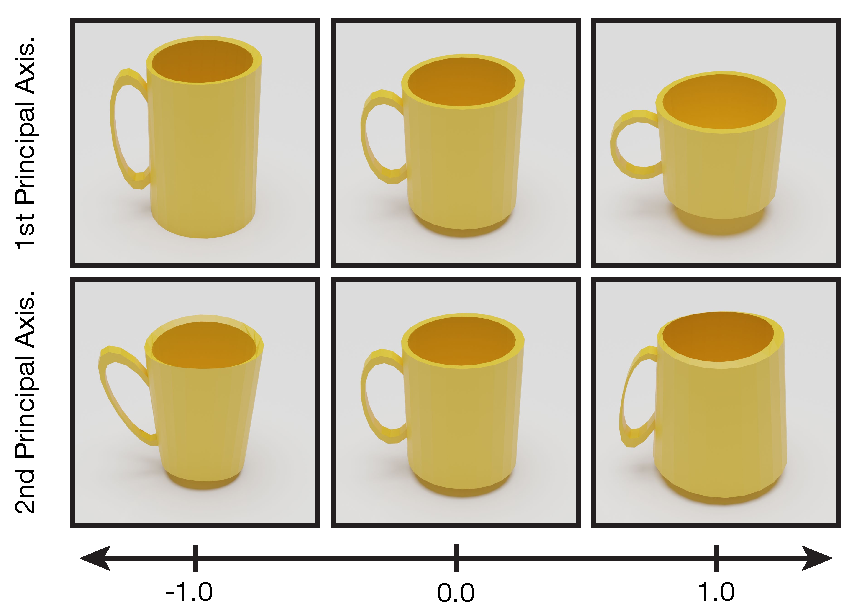
\includegraphics[width=0.45\textwidth]{figures/latent_mugs4.pdf}
%     \caption{The first two principal components of a latent space of mug warps.}
%     \label{fig:latent}
% \end{wrapfigure}

% We pre-train IW with a small number of example objects (ten objects from ShapeNet \cite{chang15shapenet} in our experiments) for each object class. We assume to have access to object meshes and we sample a point cloud per object using surface sampling. For each class, we select a canonical example $C$ that appears to be the most representative (we describe two possible heuristics in Appendix \ref{appendix:method:canonical}). Then, we apply the method of \cite{rodriguez18transferring} described in Section \ref{sec:background} to learn a latent space of object warps (Figure \ref{fig:latent}). As a result, we can parameterize object shape by a low-dimensional vector $v \in \mathbb{R}^d$ that represents the linear displacements of points in the canonical point cloud $\pcc \in \mathbb{R}^{n \times 3}$,
% \begin{align}
%     \pcx{v} = \pcc + \mathrm{Reshape}(W v). \label{eq:warp}
% \end{align}

% For motion planning on a physical robot, we found it important to have access to the surface of the object shape parameterized by $v$ in addition to its point cloud. If the point cloud of $\pcx{v}$ is dense enough, it is possible to use surface completion methods. But, we found a simpler approach to work well: we construct the canonical point cloud $\pcc$ as a concatenation of the actual vertices of object $C$ and points sampled on its surface. By having actual vertices in $\pcc$, we ensure that they can be warped to create a new mesh. We add the surface samples to make the point cloud more uniform -- meshes modeled by people tend to have highly non-uniform distributions of vertices.

% Finally, we create a new mesh by extracting the warped vertices from $\pcx{v}$ and keeping the original faces (represented as triplets of vertex indices) from object $C$. This way of warping vertices can possibly break the mesh (e.g. by intersecting or inverting its faces), but we did not find it to be a problem when performing collision checking for a reasonable range of real-world objects.

% --

% ## Pre-training

% \rob{This section seems like a recapitulation of what should be in sect 3. If there is some diff between how you're doing object warping and how it was done int he CPD paper, you should focus on that here.}

% \begin{figure}
%     \centering
%     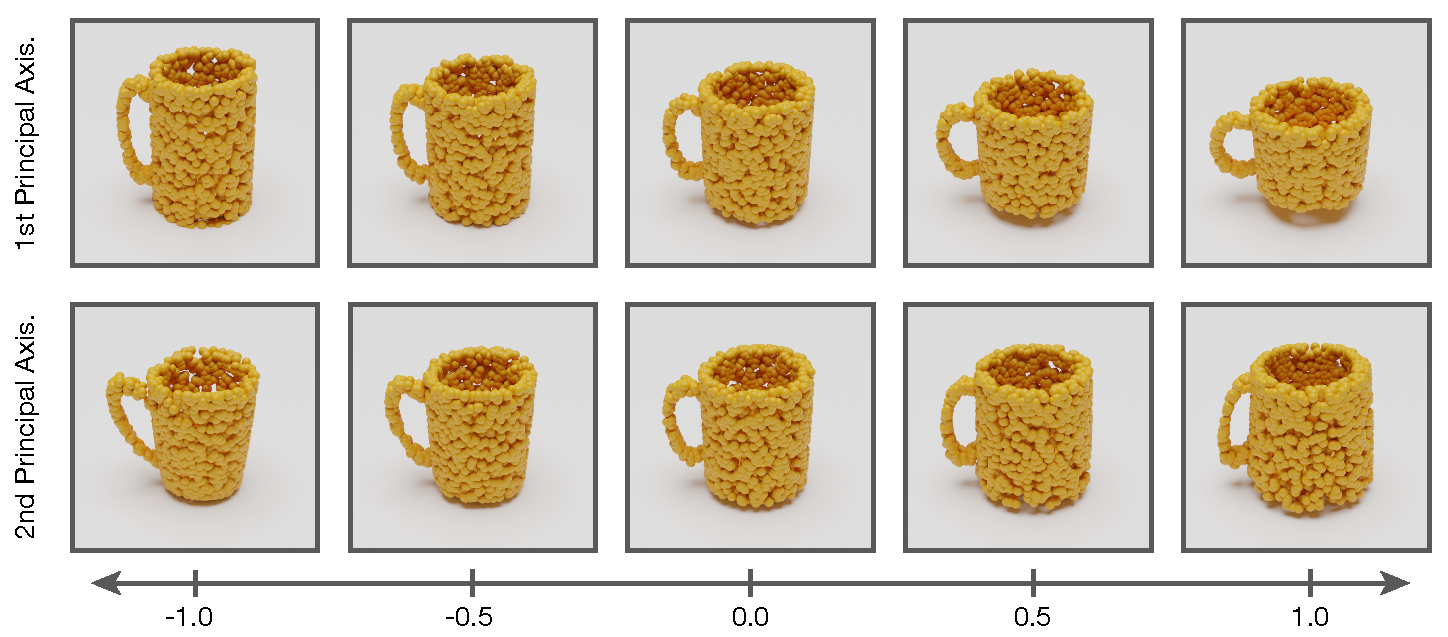
\includegraphics[width=\textwidth]{figures/latent_mugs2.pdf}
%     \caption{Traversing the latent space of warps of a canonical mug. We show the first two out of eight principal components. \ob{TODO: Show meshes instead of point cloud to reduce clutter.}}
%     \label{fig:latent}
% \end{figure}

% Our approach learns a latent space of meshes from around $K=10$ example objects per class. We outline the process in Algorithm \ref{alg:warp_learn} and describe it below. \rst{I think we should briefly mention where the meshes come from - online repositories, mesh reconstruction on a pointcloud, etc}

% We start by sampling a small point cloud $\mathrm{PCD}_i$ for each mesh using surface sampling. We then select a canonical object with index $C$ based on the point cloud dataset. The canonical object is chosen based on the ability to be warped to the other $K-1$ point clouds using Coherent Point Drift []. \rst{I was using the chamfer distance between pointclouds before warping (the summed distance between closest points in the two pointclouds) - is this something different?} We describe point cloud warping in Section \ref{sec:background}. We save the vertices and faces of the canonical object mesh, and create a concatenated point cloud, where the first $N$ points are the vertices and the remaining points are sampled on the surface of the object. We roughly maintain a 1-to-1 ratio between these two sources of points.  However, the placement of vertices can often be biased (e.g. some mug models have 90\% of their vertices in the handle); therefore, we sample additional surface points to increase uniformity.By warping vertices, we retain the ability to reconstruct the mesh. \rst{I think this bit could use emphasis over explanations of CPD since it's novel. Add why this is important - to enable contact warping/motion planning/etc}  We call the larger canonical point cloud $\mathrm{canon}$. 

% To create a latent space of warps, we warp $\mathrm{canon}$ to each point cloud in $D_W$ using Coherent Point Drift. As a result, we get a matrix of displacements $W_{C \rightarrow i}$ for each object $i$. The size of all of these matrices is $|\mathrm{canon}|{\times}3$ and they express how each point in $\mathrm{canon}$ should be translated to match the $i$th object. We flatten these matrices to create a dataset of displacements $D_W$.

% Finally, we apply PCA to $D_W$ and retain the first $L$ components to define a latent space of canonical point displacements. The latent space is linear but surprisingly expressive, as each point in $\mathrm{canon}$ can move independently in a different direction. Given an $L$-dimensional vector $v$, we can create a mesh parameterized by this vector:
% \begin{align}
%     \mathrm{canon} +\mathrm{PCA.inverse\_transform}(v)\mathrm{.reshape(-1, 3)}.
% \end{align}
% The first $N$ warped points in $\mathrm{canon}$ are the vertices of the mesh and the faces remain the same across warps. 

% ## Perception

% \tk{The title of this section says "Perception": I would expect some information about how we go from the camera images (which you show in the figures) to the 3D point cloud / mesh representation of individual objects}

% Given an observed, possibly partial, point cloud $\mathrm{pcd}$, our goal is to predict the latent shape $v$ and pose $T$ of the object. We describe this in Algorithm \ref{alg:warp_infer}.

% \rob{Now, we're getting into material that is novel to this paper. If the objective here can be expressed mathematically (e.g. in terms of min and max), that would be nice. Talk about *what* we're doing mathematically. then talk about how we're doing it -- SGD and random restarts.}

% To jointly estimate the pose and shape, we employ a gradient-based optimization approach with multiple random starts. For each random start, we sample a random $3D$ rotation and use fixed initialization for latent shape $v$, translation $t_{\mathrm{local}}$ and scale $s$. We reconstruct a point cloud using $v$, scale it using $s$, and transform it using the rotation and translation. We then calculate the difference between the reconstructed and predicted point cloud and take a gradient descent step with respect to shape, scale and pose using the Adam optimizer []. We also add a regularizer on the size of the reconstructed object controlled by a hyper-parameter $\beta$.

% We use multiple random restarts with different initial rotations because the joint optimization of shape and pose is prone to local minima. For example, if the optimizer cannot align the handle of the mug with the observed point cloud due to an unfavorable random start, it might instead choose to make the handle as small as possible. This behavior is fixed by taking the parameters of the object with the best fit across many random initial rotations.

% \rob{Agree w/ everything Elise says below. Maybe say explicitly what GS does and how BP works there. Cite others who use GS this way.}

% Another problem is the gradient descent with respect to 3D rotations. While previous approaches have directly optimized Euler angles [], which can be tricky \evdp{better to explicitly explain issues e.g. singularities}, we choose a more elegant \evdp{should not call our own approach elegant} approach of directly learning the 3D rotation matrix []. We parameterize the rotation matrix as a $2{\times}3$ matrix $r$ and perform Gram-Schmidt orthogonalization [], which creates a 3D rotation matrix. This process can be backpropagated through to update $r$. \evdp{does having to backpropagate through GS make training expensive? It might be good to add some information about training wall clock time}

% \begin{table}[h]
%     \centering
%     \begin{tabular}{lccc}
%         \toprule
%          \textbf{Method} & \# Train. Objects & \# Demos. & Labels \\
%          \midrule
%          NDF & 200 & 5-10 & Yes \\
%          R-NDF & 200 & 5-10 & Yes \\
%          TAX-Pose & 200 & 5-10 & No \\
%          \textbf{SA-Warp} & \textbf{10} & \textbf{1} & \textbf{No} \\
%          \bottomrule
%     \end{tabular}
%     \caption{Required training objects, training demonstrations and additional labeled data across methods.}
%     \label{tab:training}
% \end{table}

% \begin{figure*}[]
%     \centering
%     \begin{subfigure}{(\linewidth - 0.1\linewidth)/6}
%         \centering
%         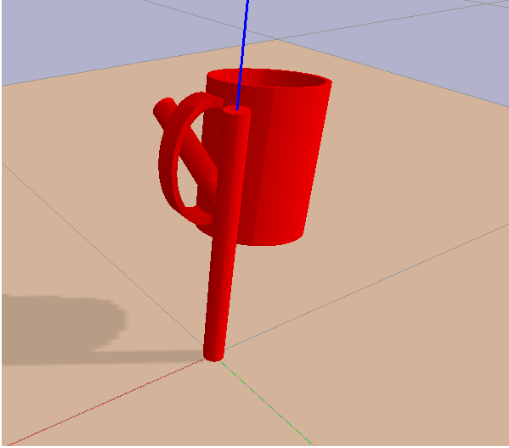
\includegraphics[width=\linewidth]{figures/virtual/1.png}
%         \caption{}
%     \end{subfigure}
%     \begin{subfigure}{(\linewidth - 0.1\linewidth)/6}
%         \centering
%         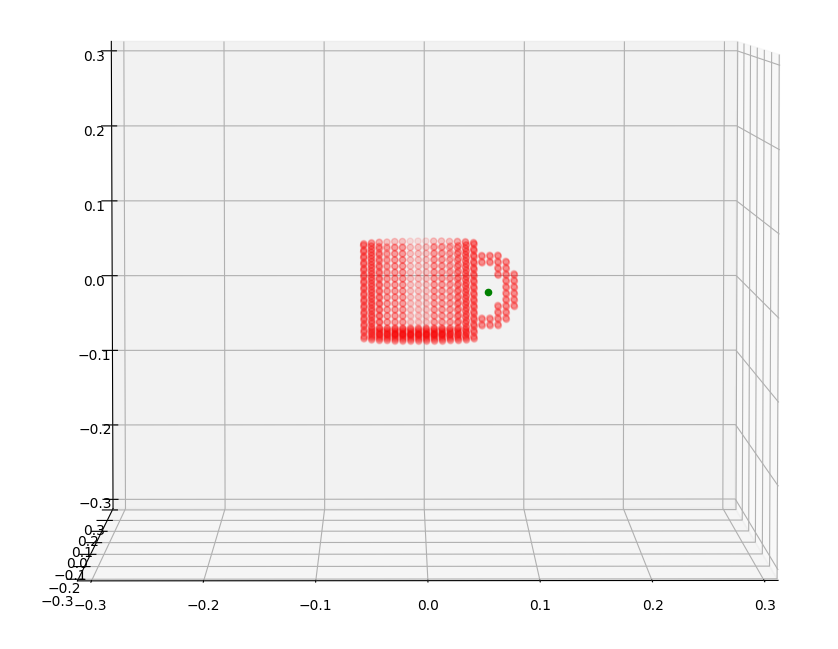
\includegraphics[width=\linewidth]{figures/virtual/2.png}
%         \caption{}
%     \end{subfigure}
%     \begin{subfigure}{(\linewidth - 0.1\linewidth)/6}
%         \centering
%         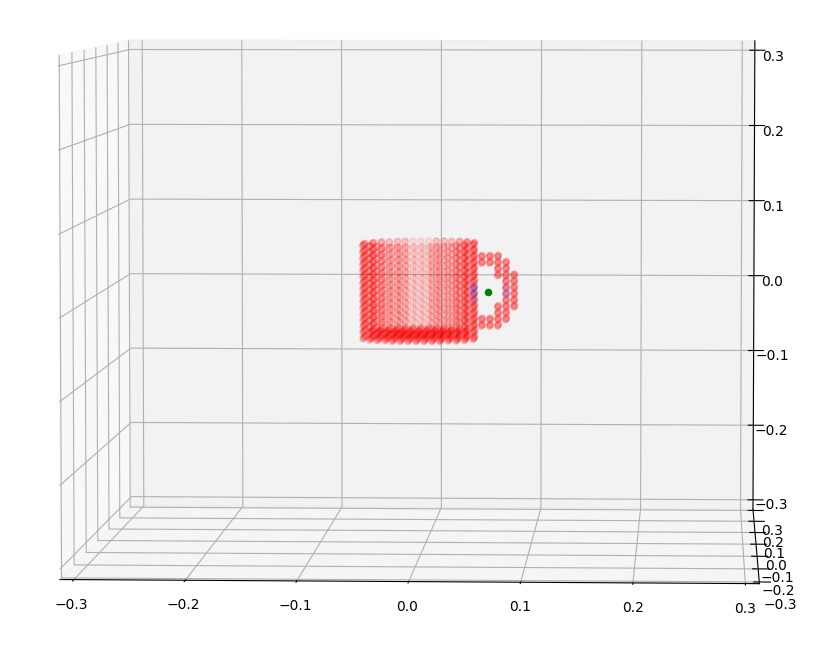
\includegraphics[width=\linewidth]{figures/virtual/3.png}
%         \caption{}
%     \end{subfigure}
%     \begin{subfigure}{(\linewidth - 0.1\linewidth)/6}
%         \centering
%         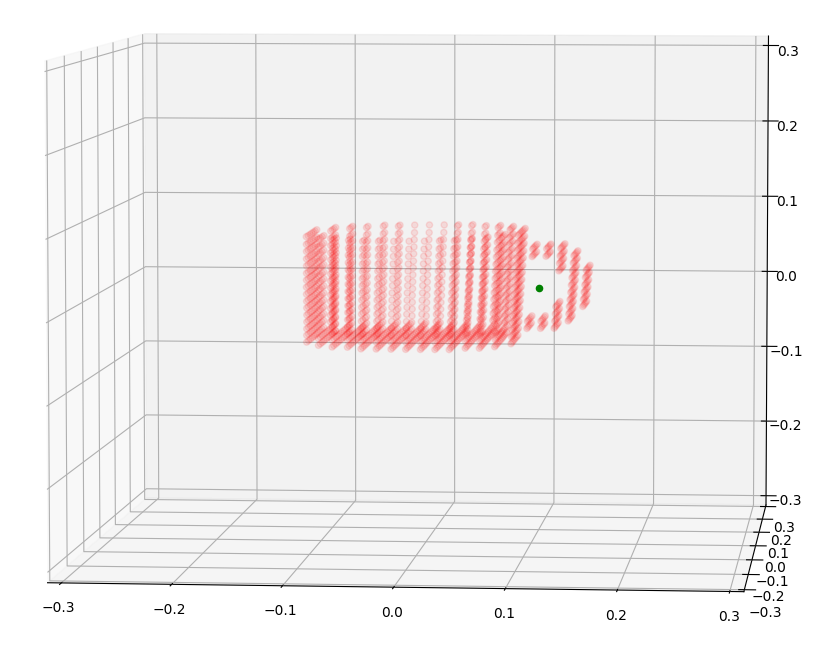
\includegraphics[width=\linewidth]{figures/virtual/4.png}
%         \caption{}
%     \end{subfigure}
%     \begin{subfigure}{(\linewidth - 0.1\linewidth)/6}
%         \centering
%         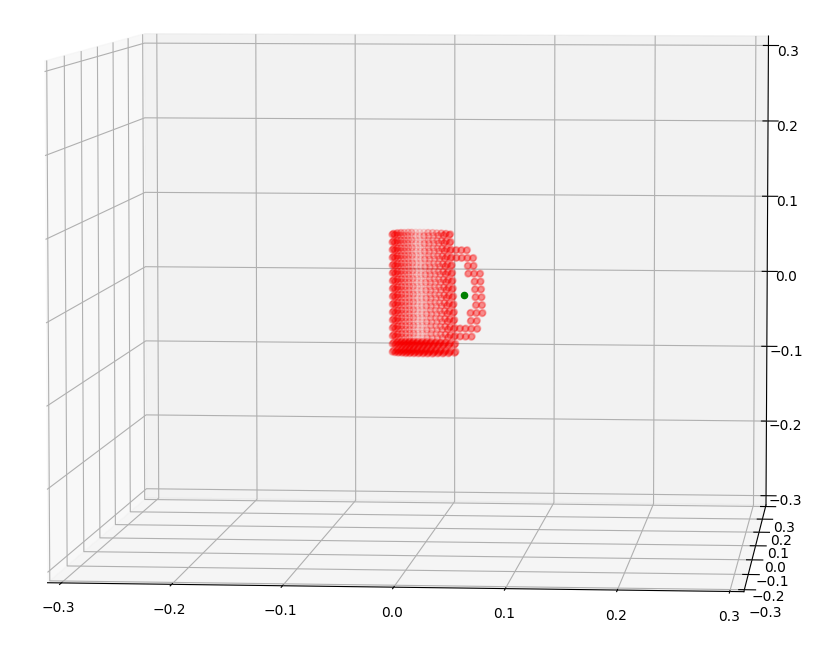
\includegraphics[width=\linewidth]{figures/virtual/5.png}
%         \caption{}
%     \end{subfigure}
%     \begin{subfigure}{(\linewidth - 0.1\linewidth)/6}
%         \centering
%         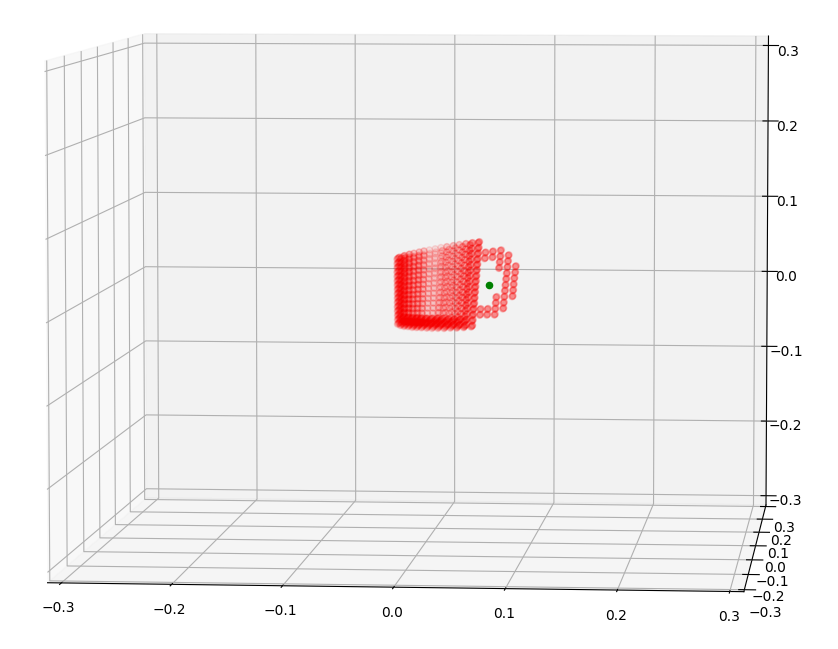
\includegraphics[width=\linewidth]{figures/virtual/6.png}
%         \caption{}
%     \end{subfigure}
%     \caption{Sketch: (a): a demonstration of the mug tree task, (b) a virtual point (green) in the middle of the mug's handle, (c) 10 (?) nearest neighbors (blue\ob{almost invisible, I know}), (d-f) warping the virtual point together with the mug.}
%     \label{fig:virtual_points}
% \end{figure*}

% # Limitations

% \begin{itemize}
%     \item We run joint shape warping and pose estimation using gradient descent and many random restarts. This process takes around 25 seconds per object on a single desktop GPU. Future work could train an additional neural network to skip the gradient descent, or to predict favorable initialization.
%     \item Shape warping represented using PCA cannot capture the detail of each object. Tasks that require a high-degree of precision might have a low success rate. But, PCA can be easily replaced with a higher capacity model (which might require more than 10 training meshes per object class).
%     \item Our method does not learn from its failures; its behavior is fully determined by the shape warping model and a single demonstration. But, the entire prediction process, from shape warping to interaction point cloning, is technically fully differentiable.
%     \item While relatively robust to partial and noisy point clouds, our method cannot reason about object parts that are not shown in the point cloud. For example, our method currently cannot infer that a handle of a mug is occluded by the mug itself if it is not shown in the point cloud. It would instead predict an arbitrary orientation of the mug.
% \end{itemize}
